%!TEX root = ../thesis_a4.tex
% Some new commands for setting up appendices
\newcommand\contrib[1]{\\~{\footnotesize (#1)}}
% 
\newcommand\resource[2]{
	\noindent #1 \par
	\vspace{0.2em}
	{\centering	\url{#2} \par}
	\vspace{0.5em}
	\hrule \par 
	\vspace{0.8em} \par}
%
%
\chapter[Publications by the Author][Publications by the Author]{Publications by the Author}
\label{app:mypapers}% by the author

We here provide a list of publications by the author related with the thesis work. For the publications where the role is not that of the first author we  also specify the contributions. Wherever not specified, the contributions are mainly in the formulation of the research problem, building the dataset, writing the code, performing the experiments, analyzing the results and writing the manuscript.

\subsection*{Peer-reviewed journals}
\begin{itemize}[leftmargin=*]
	\item \textbf{Gulati, S.}, Bellur, A., Salamon, J., Ranjani, H., Ishwar, V., Murthy, H. A., \& Serra, X. (2014). Automatic tonic identification in Indian art music: approaches and evaluation. \textit{Journal of New Music Research}, 43(1), 53–71.
	\contrib{Companion webpage: \url{http://compmusic.upf.edu/node/323}}
	\item Koduri, G. K., \textbf{Gulati, S.}, Rao, P., \& Serra, X. (2012). R\={a}ga recognition based on pitch distribution methods. \textit{Journal of New Music Research}, 41(4), 337–350.
	\contrib{Formulating methodology, Writing parts of the code}
	
\end{itemize}
%
\subsection*{Full articles in peer-reviewed conferences}
\begin{itemize}[leftmargin=*]
	\item \textbf{Gulati, S.}, Serr{\`a}, J., Ganguli, K. K., \c{S}ent{\"u}rk, S., \& Serra, X. (2016). Time-delayed melody surfaces for r\={a}ga recognition. In \textit{Proceedings of the 17th International Society for Music Information Retrieval Conference (ISMIR)}, pp. 751–757. New York, USA.
	\contrib{Companion webpage: \url{http://compmusic.upf.edu/node/300}}
	%
	\item Ganguli, K. K., \textbf{Gulati, S.}, Serra, X., \& Rao, P. (2016). Data-driven exploration of melodic structures in Hindustani music. In \textit{Proceedings of the 17th International Society for Music Information Retrieval Conference (ISMIR)}, pp. 605-611. New York, USA.
	\contrib{Formulation of the problem, building dataset, writing the code, writing the manuscript.}
	%
	\item \textbf{Gulati, S.}, Serr{\`a}, J., Ishwar, V., \c{S}ent{\"u}rk, S., \& Serra, X. (2016). Phrase-based r\={a}ga recognition using vector space modeling. In \textit{Proceedings of the 41st IEEE International Conference on Acoustics, Speech and Signal Processing (ICASSP)} , pp. 66–70. Shanghai, China.
	\contrib{Companion webpage: \url{http://compmusic.upf.edu/node/278}}
	%
	\item \textbf{Gulati, S.}, Serr{\`a}, J., Ishwar, V., \& Serra, X. (2016). Discovering r\={a}ga motifs by characterizing communities in networks of melodic patterns. In \textit{Proceedings of the 41st IEEE International Conference on Acoustics, Speech and Signal Processing (ICASSP)}, pp. 286–290. Shanghai, China.
	\contrib{Companion webpage: \url{http://compmusic.upf.edu/node/277}}
	%
	\item \textbf{Gulati, S.}, Serr{\`a}, J., \& Serra, X. (2015). Improving melodic similarity in Indian art music using culture-specific melodic characteristics. In \textit{Proceedings of the 16th International Society for Music Information Retrieval Conference (ISMIR)}, pp. 680–686. M{\'a}laga, Spain.
	\contrib{Companion webpage: \url{http://compmusic.upf.edu/node/269}}
	%
	\item \textbf{Gulati, S.}, Serr{\`a}, J., \& Serra, X. (2015). An evaluation of methodologies for melodic similarity in audio recordings of Indian art music. In \textit{Proceedings of the 40th IEEE International Conference on Acoustics, Speech and Signal Processing (ICASSP)}, pp. 678–682. Brisbane, Australia.
	\contrib{Companion webpage: \url{http://compmusic.upf.edu/node/242}}
	%
	\item \textbf{Gulati, S.},  Serr{\`a}, J., Ishwar, V., \& Serra, X. (2014). Mining melodic patterns in large audio collections of Indian art music. In \textit{Proceedings of the International Conference on Signal Image Technology \& Internet Based Systems (SITIS-MIRA)}, pp. 264–271. Marrakesh, Morocco.
	\contrib{Companion webpage: \url{http://compmusic.upf.edu/node/210}}
	%
	\item \textbf{Gulati, S.}, Serr{\`a}, J., Ganguli, K. K., \& Serra, X. (2014). Landmark detection in Hindustani music melodies. In \textit{Proceedings of the International Computer Music Conference / Sound and Music Computing Conference (ICMC-SMC)}, pp. 1062-1068. Athens, Greece. 
	\contrib{Companion webpage: \url{http://compmusic.upf.edu/node/324}}
	%
	\item Srinivasamurthy, A., Koduri, G. K., \textbf{Gulati, S.}, Ishwar, V., \& Serra, X. (2014). Corpora for Music Information Research in Indian Art Music. In \textit{Proceedings of Joint International Computer Music Conference/Sound and Music Computing Conference}. Athens, Greece. 
	\contrib{Compilation of the research corpora. Companion webpage: \url{http://compmusic.upf.edu/smc-2014-corpora}}
	%
	\item \c{S}ent{\"u}rk, S., \textbf{Gulati, S.}, \& Serra, X. (2014). Towards alignment of score and audio recordings of Ottoman-Turkish makam music. In \textit{Proceedings of the 4th International Workshop on Folk Music Analysis (FMA)}. Istanbul, Turkey. 
	\contrib{Conceptualization, ideas and discussions}
	%
	\item Bogdanov, D., Wack, N., G{\'o}mez, E., \textbf{Gulati, S.}, Herrera, P., Mayor, O., Roma, G., Salamon, J., Zapata, J., \& Serra, X. (2013). Essentia: an audio analysis library for music information retrieval. In \textit{Proceedings of the 14th International Society for Music Information Retrieval Conference (ISMIR)}, pp. 493–498. Curitiba, Brazil.
	\contrib{Implementation of the tonic identification method in Essentia}
	%
	\item Bogdanov, D., Wack, N., G{\'o}mez, E., \textbf{Gulati, S.}, Herrera, P., Mayor, O., Roma, G., Salamon, J., Zapata, J., \& Serra, X. (2013). ESSENTIA: an open-source library for sound and music analysis. In \textit{Proceedings of the 21st ACM international conference on Multimedia}, pp. 855–858. Barcelona, Spain.
	\contrib{Implementation of the tonic identification method in Essentia}	
	%	
	\item \c{S}ent{\"u}rk, \textbf{S., Gulati, S.}, \& Serra, X. (2013). Score informed tonic identification for makam music of turkey. In \textit{Proceedings of the 14th International Society for Music Information Retrieval Conference (ISMIR)}, pp. 175–180. Curitiba, Brazil.
	\contrib{Conceptualization, ideas and discussions}
	%
	\item Sordo, M., Koduri, G. K., \c{S}ent{\"u}rk, S., \textbf{Gulati, S.}, \& Serra, X. (2012). A musically aware system for browsing and interacting with audio music collections. In \textit{Proceedings of the 2nd CompMusic Workshop}. Istanbul, Turkey.
	\contrib{Compilation of the research corpora}
	%
	\item Koduri, G. K., \textbf{Gulati, S.}, \& Rao, P. (2011). A survey of raaga recognition techniques and improvements to the state-of-the-art. In \textit{Proceedings of the Sound and Music Computing Conference (SMC)}. Padova, Italy.
	\contrib{Formulating methodology, Writing parts of the code}
	%	
\end{itemize}
%
\subsection*{Other contributions to conferences}
\begin{itemize}[leftmargin=*]
	\item \textbf{Gulati, S.},  Serr{\`a}, J., Ishwar, V., \& Serra, X. (2014). Melodic Pattern Extraction in Large Collections of Music Recordings Using Time Series Mining Techniques. In Late-Breaking Demo Session of the 15th International Society for Music Information Retrieval Conference. Taipei, Taiwan. 
	%
	\item \textbf{Gulati, S.}, Ganguli, K. K., Gupta, S., Srinivasamurthy, A., \& Serra, X. (2015). \gls{ragawise}: A Lightweight Real-time Raga Recognition System for Indian Art Music. In Late-Breaking Demo Session of the 16th International Society for Music Information Retrieval Conference. Malaga, Spain. 
	\contrib{Companion webpage: \url{http://compmusic.upf.edu/node/281}}
	%
	\item Caro, R., Srinivasamurthy, A., \textbf{Gulati, S.}, \& Serra, X. (2014). Jingju music: Concepts and Computational Tools for its Analysis. A Tutorial in the 15th International Society for Music Information Retrieval Conference, Taipei, Taiwan. 
	\contrib{Presented the melody part of the tutorial, focused on melodic analysis tools for {jingju} music. Companion webpage:  \url{http://compmusic.upf.edu/jingju-tutorial}}
	
\end{itemize}



%%%%%%%%%%%%%%%%%%%%%%%%%%%%%%%%%%%%%%%%%%%%%%%%%%%%%%%%%%%%%%%%%%%%%%%%%%%%%%
%%%%%%%%%%%%%%%%%%%%%%%%%%%%%%%%%%%%%%%%%%%%%%%%%%%%%%%%%%%%%%%%%%%%%%%%%%%%%%

\chapter{Resources}\label{app:resources}

In this appendix, we provide the URLs to access the resources related to this thesis, which include the code and tools, the corpora and test datasets, and the applications and demos. An up-to-date links of all these resources are maintained on the companion web page of this thesis: \url{http://compmusic.upf.edu/node/304} (mirrored at \url{http://www.sankalpgulati.in/phd-thesis.html}).

\section*{Code and Tools}

\subsection*{Implementation of Methods}
Implementation of the methods presented in this thesis are made publicly available for research purposes. We also indicate (in squared brackets) the language in which the implementation is available.

\begin{itemize}
	\item Tonic identification (\acrshort{tonicid_justin}) [C]
	\item \Gls{nyas} segmentation and classification [Python]
	\item Predominant pitch post-processing [Python]
	\item \Gls{tani} Segmentation [Python]
	\item Pattern processing: melodic similarity, and pattern search and discovery (including cascaded lower-bound computations) [C]
	\item \Gls{dtw} variants [C, Python-wrapper]
	\item Melodic pattern characterization [Python]
	\item \Gls{raga} recognition using melodic patterns (\acrshort{ragarecVSM}) [Python]
	\item \Gls{raga} recognition using \acrshort{tdms} (\acrshort{ragarecTDMS}) [Python]
	\item Pitch estimation using the YIN algorithm [JavaScript]
\end{itemize}

\subsection*{Tools}

\begin{itemize}
	\item Essentia audio analysis library (\url{http://essentia.upf.edu/})
	\item Dunya API  (\url{https://github.com/MTG/pycompmusic})
	\item Dunya front end  (\url{http://dunya.compmusic.upf.edu/})
	\item Dunya server and back end  (\url{https://github.com/MTG/dunya})
\end{itemize}


\section*{Corpora and Test-datasets}

\subsection*{Corpora}

All the research corpora described in this thesis, which include audio recordings, associated metadata and audio features can be accessed through the Dunya \acrshort{api} (\secref{sec:applications_dunya}). Every corpora has a corresponding collection in MusicBrainz.

\begin{itemize}
	\item `Dunya Carnatic' collection in MusicBrainz forms the Carnatic music corpus (\secref{sec:corpus_carnatic_music_corpus}) \\ \url{https://musicbrainz.org/collection/f96e7215-b2bd-4962-b8c9-2b40c17a1ec6}
	\item `Dunya Hindustani' collection in MusicBrainz forms the Hindustani music corpus (\secref{sec:corpus_carnatic_music_corpus}) \\
	\url{https://musicbrainz.org/collection/213347a9-e786-4297-8551-d61788c85c80}
	\item `Dunya Carnatic CC' and `Dunya Hindustani CC' collection in MusicBrainz forms the open-access music corpus (\secref{sec:corpus_open_access_research_corpus}) \\
	\url{https://musicbrainz.org/collection/a163c8f2-b75f-4655-86be-1504ea2944c2}\\
	\url{https://musicbrainz.org/collection/6adc54c6-6605-4e57-8230-b85f1de5be2b}
\end{itemize}

\subsection*{Test Datasets}

All the test datasets described in this thesis are shared as standalone archives (files) that contain relevant annotations and audio features. For the datasets that use audio recordings present in the corpora, the recordings can be accessed though the Dunya \acrshort{api}. Otherwise, they are bundled together with the annotations. List of all the datasets which are made publicly available.
\begin{itemize}
	\item Tonic identification datasets (\acrshort{tds_cm1}, \acrshort{tds_cm2}, \acrshort{tds_cm3}, \acrshort{tds_iitm1}, \acrshort{tds_iitm2}, and \acrshort{tds_iisc})
	\item \Gls{nyas} detection dataset (\acrshort{nds_cm})
	\item Melodic similarity datasets (\acrshort{msds_iitm_cmd}, \acrshort{msds_iitb_hmd}, \acrshort{msds_cm_cmd}, and \acrshort{msds_cm_hmd})
	\item \Gls{raga} recognition datasets (\acrshort{rrds_cmd_big} and \acrshort{rrds_hmd_big})
\end{itemize}

The corpora and the test datasets compiled in the CompMusic project for all the music traditions are available at:
\begin{description}[style=nextline]
	\item[CompMusic music corpora] \url{http://compmusic.upf.edu/corpora}
	\item[CompMusic test datasets] \url{http://compmusic.upf.edu/datasets}
\end{description}


\section*{Applications, and Demos}

\begin{itemize}
	\item Discovered melodic patterns:
	\begin{itemize}
		\item Metadata-wise browsing: \url{dunya.compmusic.upf.edu/motifdiscovery}
		\item Network of melodic patterns: \url{dunya.compmusic.upf.edu/pattern_network/}
		\item We also share the database of the discovered melodic patterns that contains the time-stamps, similarity with the other patterns, and the corresponding recording information for all the patterns.
	\end{itemize}
	\item \gls{ragawise}:
	\begin{itemize}
		\item Web interface: \url{https://dunya.compmusic.upf.edu/ragawise/}
		\item Code: \url{https://github.com/sankalpg/ragawise}
	\end{itemize}
	
	\item Mobile applications:
	\begin{itemize}
		\item \Gls{saraga}: \url{https://play.google.com/store/apps/details?id=com.musicmuni.saraga}
		\item \Gls{riyaz}: \url{https://play.google.com/store/apps/details?id=com.musicmuni.riyaz}
	\end{itemize}
\end{itemize}

We reiterate that the links provided for some of these resources may change over time. An up-to-date links of all these resources are maintained on the companion web page of this thesis: \url{http://compmusic.upf.edu/node/304} (mirrored at \url{http://www.sankalpgulati.in/phd-thesis.html}).

%%%%%%%%%%%%%%%%%%%%%% Another appendix!  %%%%%%%%%%%%%%%%%%%

\chapter{Additional Figures and Tables}
\label{app:additional_material}

	
\begin{figure}[h]
	\begin{subfigure}{\textwidth}
		\centering
		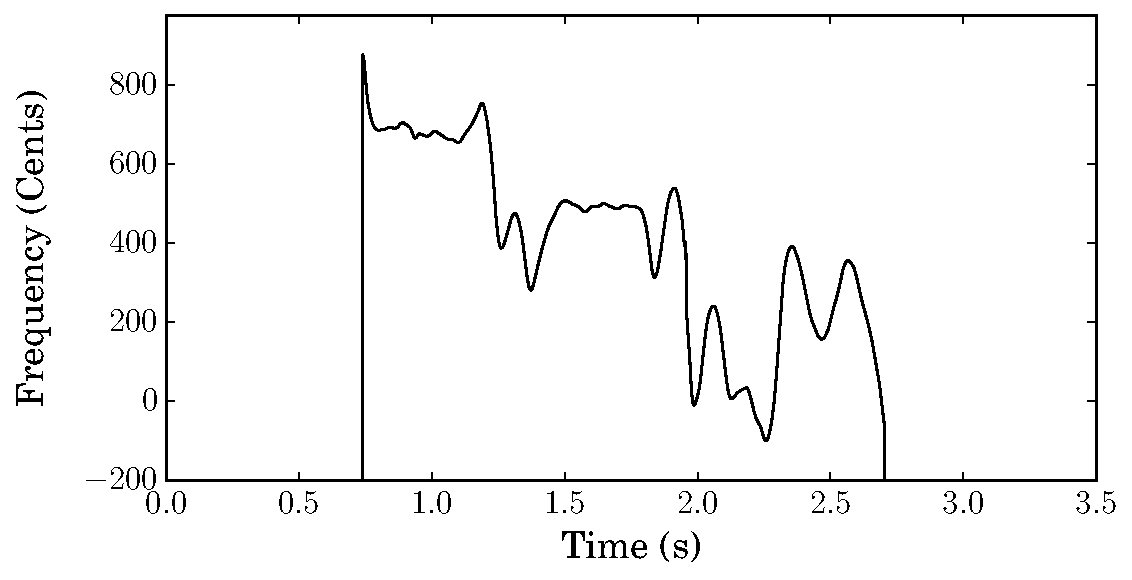
\includegraphics[width=\figSizeSeventy]{ch02_background/figures/Sphuritam_on_M1_Raga_Arabhi.pdf}
		\caption{\Gls{sphuritam} \gls{gamaka}\protect\footnotemark}
		\label{fig:sphuritam_todi}
	\end{subfigure}
	\begin{subfigure}{\textwidth}
		\centering		
		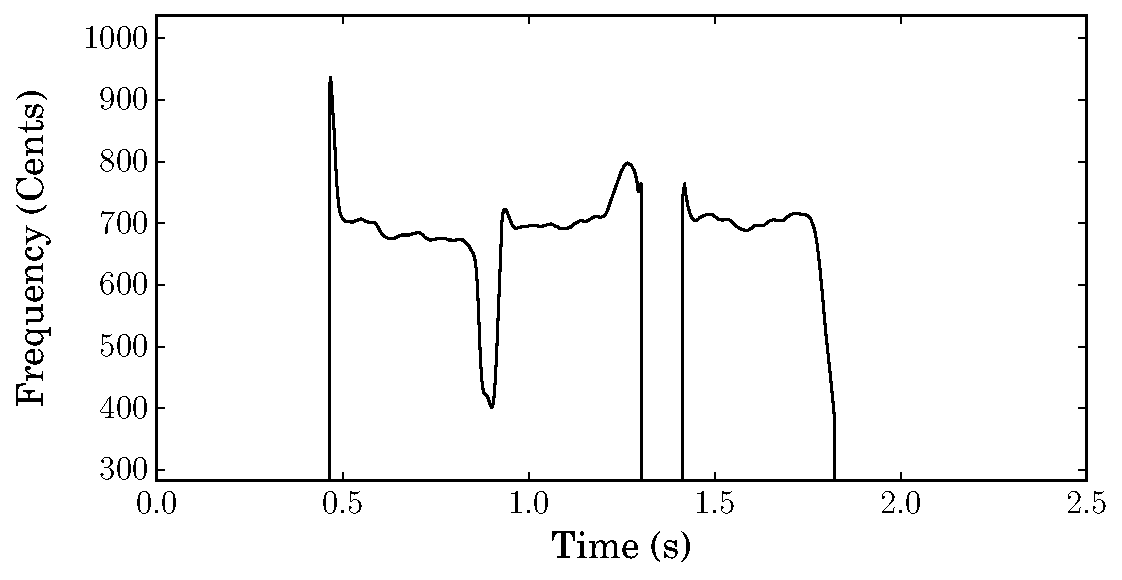
\includegraphics[width=\figSizeSeventy]{ch02_background/figures/Odukkal_on_D1.pdf}
		\caption{\Gls{odukkal} \gls{gamaka}\protect\footnotemark}
		\label{fig:odukkal_todi}
	\end{subfigure}
	\caption[Examples of \gls{gamaka} in Carnatic music]{Examples of the \gls{sphuritam} and \gls{odukkal} \gls{gamaka} in Carnatic music}
	\label{fig:example_sphuritam_odukkal}
\end{figure}
\footnotetext[1]{\url{https://www.freesound.org/people/sankalp/sounds/360769/}}
\footnotetext{\url{https://www.freesound.org/people/sankalp/sounds/360770/}}



\begin{figure}
	\begin{center}
		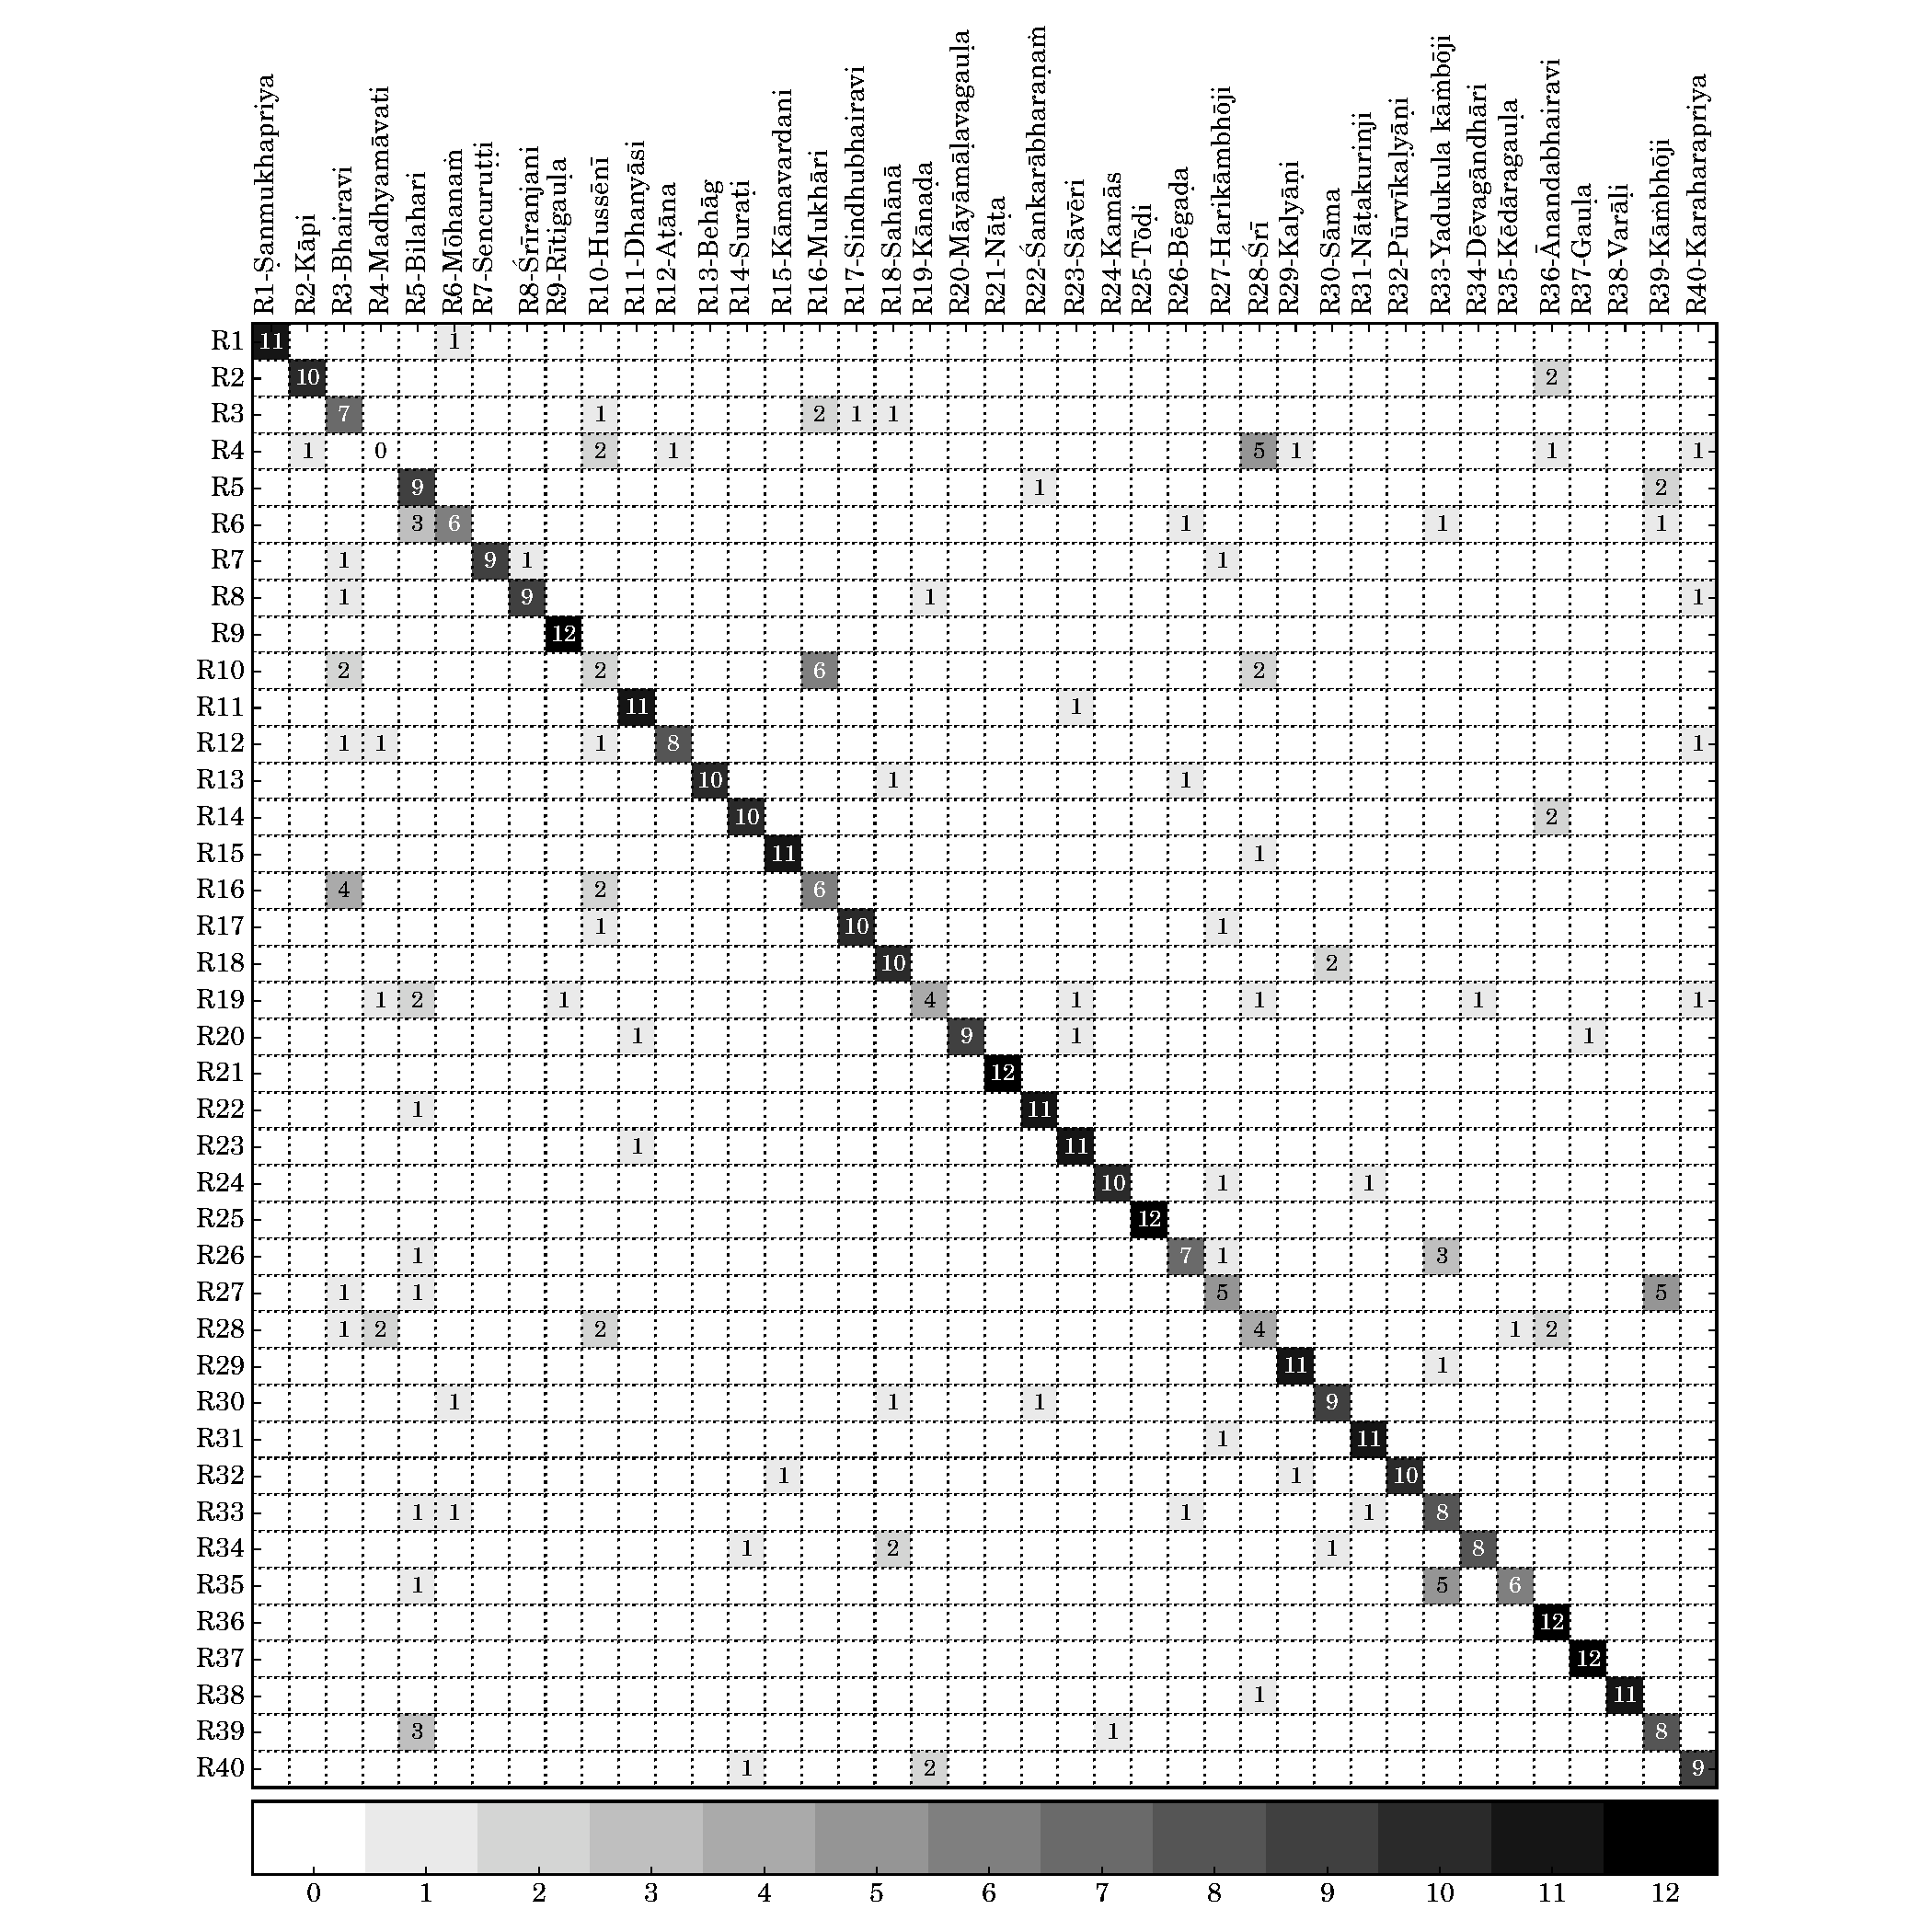
\includegraphics[width=\figSizeHundred]{ch07_ragaRecognition/figures/CM_pcd_cmd.pdf}
	\end{center}
	\caption[Confusion matrix of the classification results by \acrshort{sotaChordia} on \acrshort{rrds_cmd_big}]{Confusion matrix of the \gls{raga} predictions by \acrshort{sotaChordia} on \acrshort{rrds_cmd_big} dataset. The different shades of grey are mapped to different number of audio recordings.}
	\label{fig:confusion_matrix_cmd_chordia}
\end{figure}


\begin{figure}
	\begin{center}
		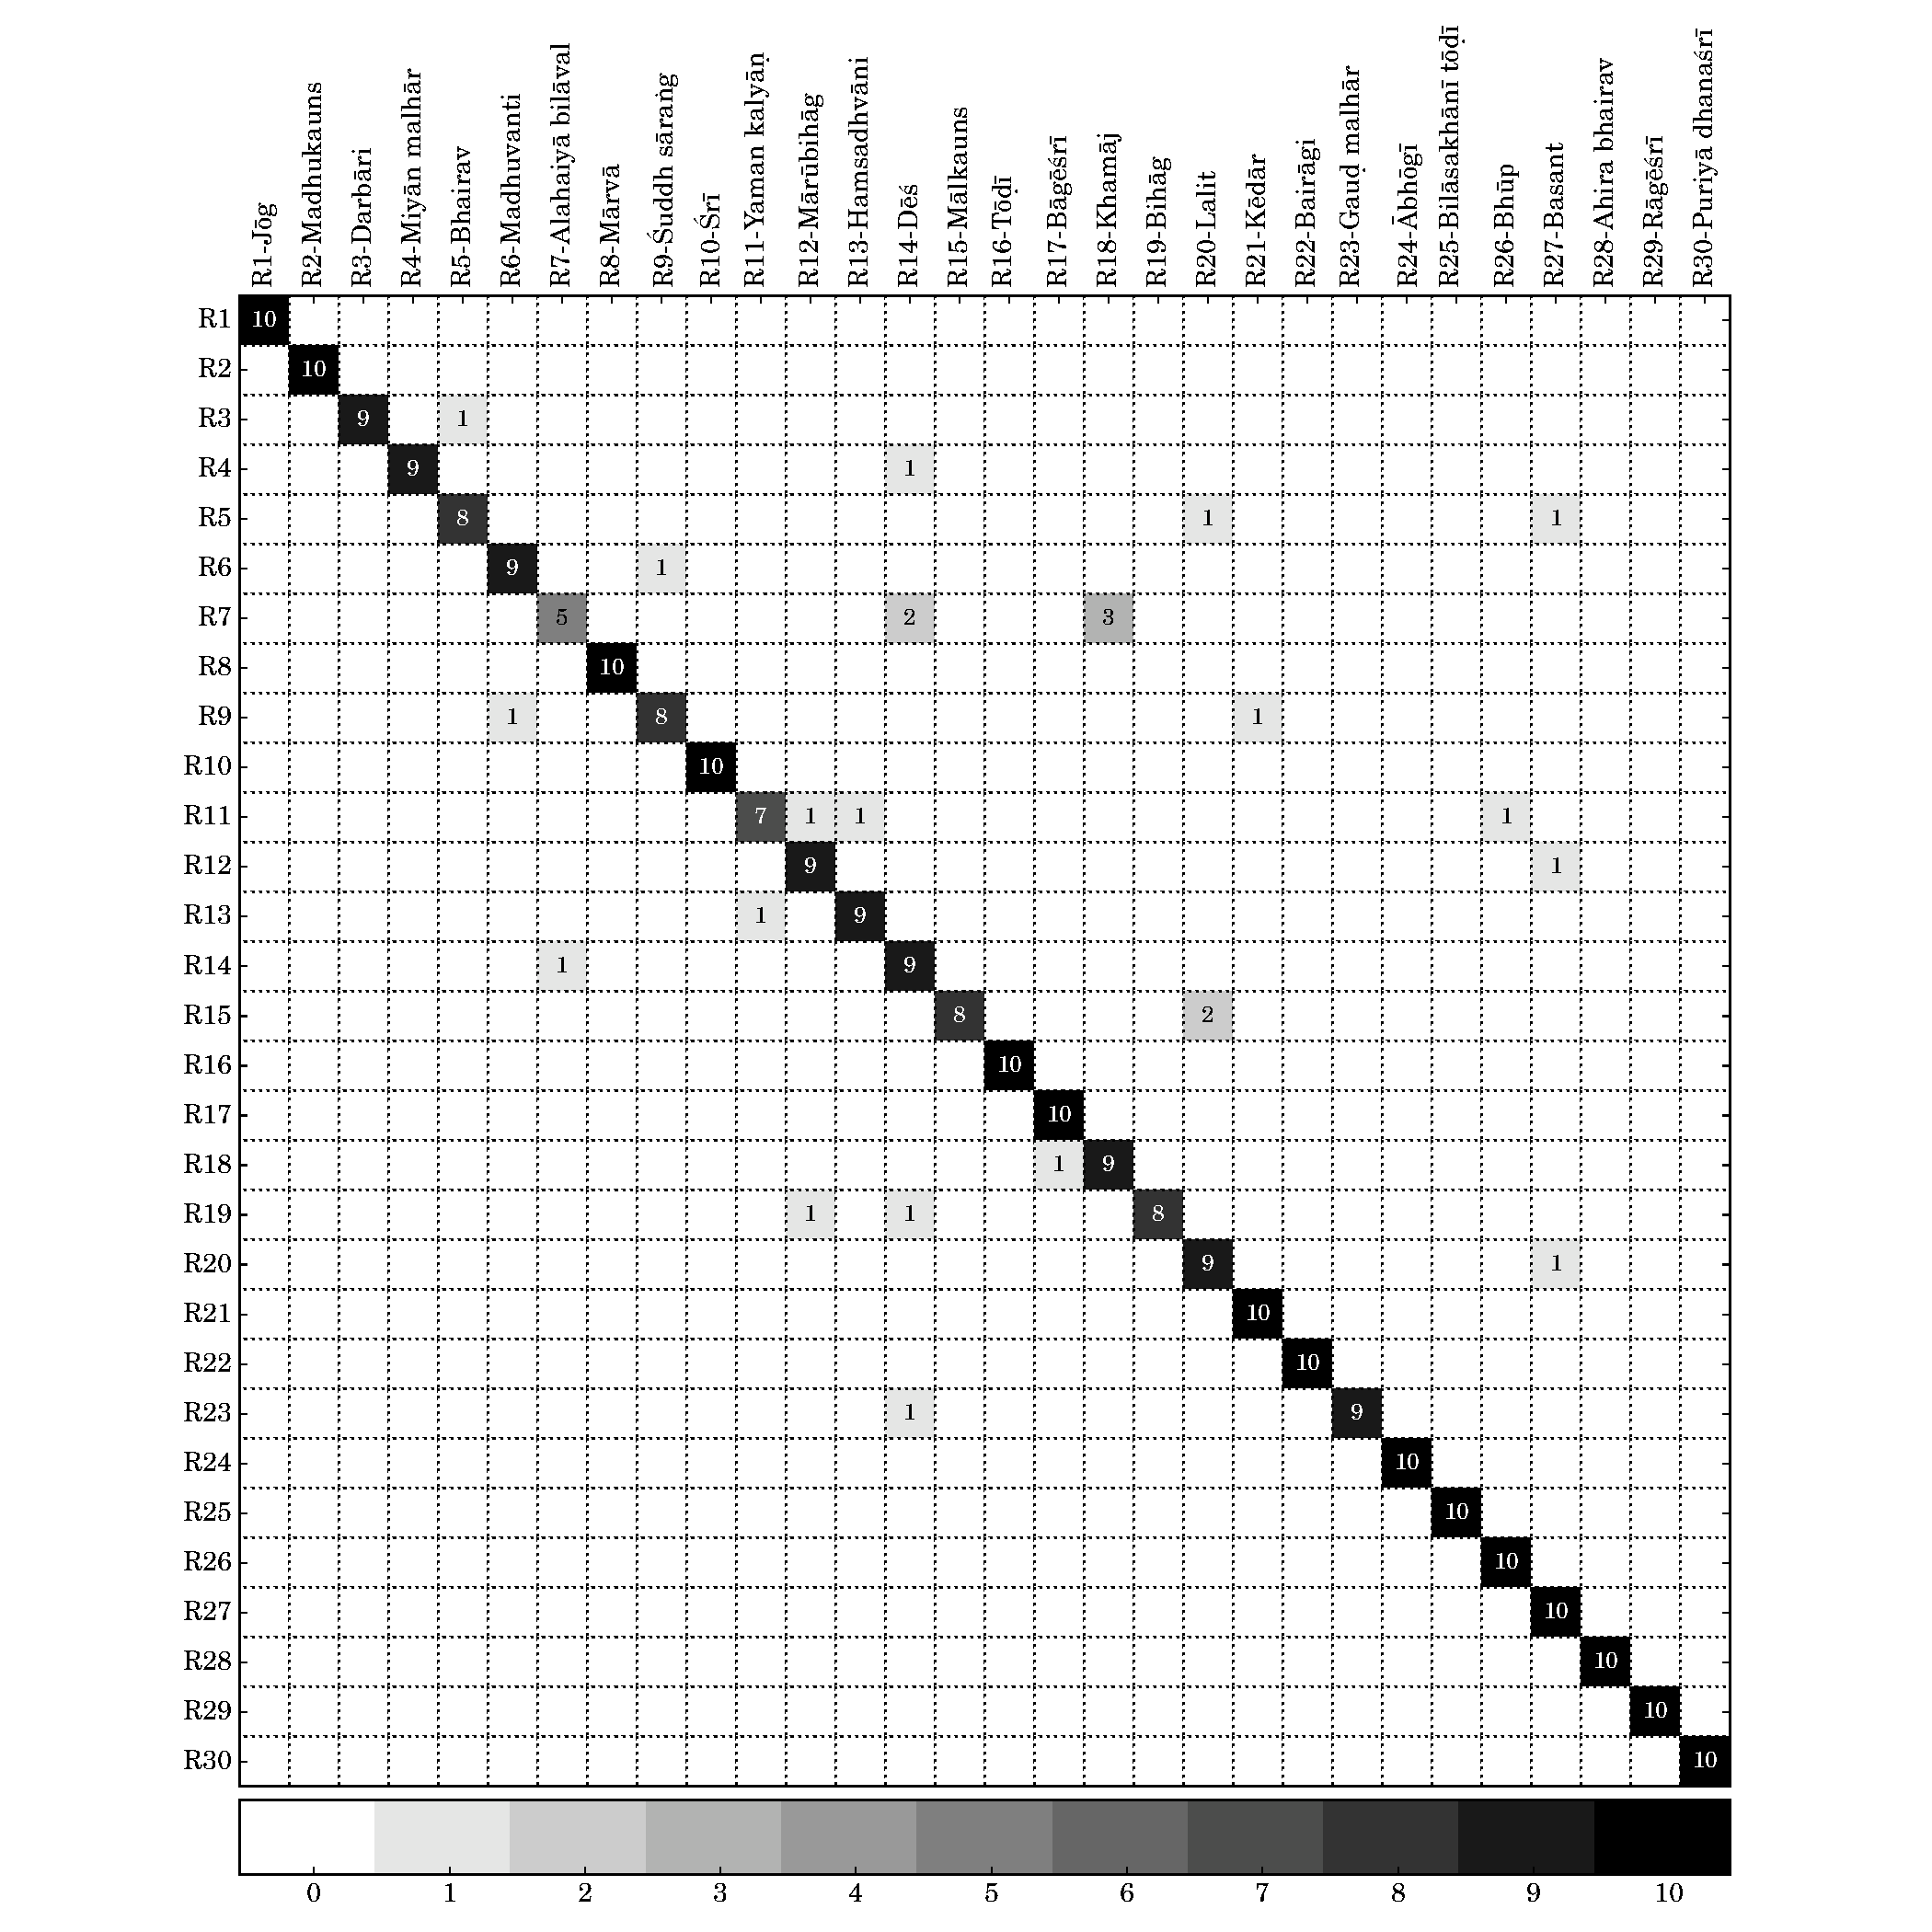
\includegraphics[width=\figSizeHundred]{ch07_ragaRecognition/figures/CM_pcd_hmd.pdf}
	\end{center}
	\caption[Confusion matrix of the classification results by \acrshort{sotaChordia} on \acrshort{rrds_hmd_big}]{Confusion matrix of the \gls{raga} predictions by \acrshort{sotaChordia} on \acrshort{rrds_hmd_big} dataset. The different shades of grey are mapped to different number of audio recordings.}
	\label{fig:confusion_matrix_hmd_chordia}
\end{figure}



\begin{figure}
	\begin{center}
		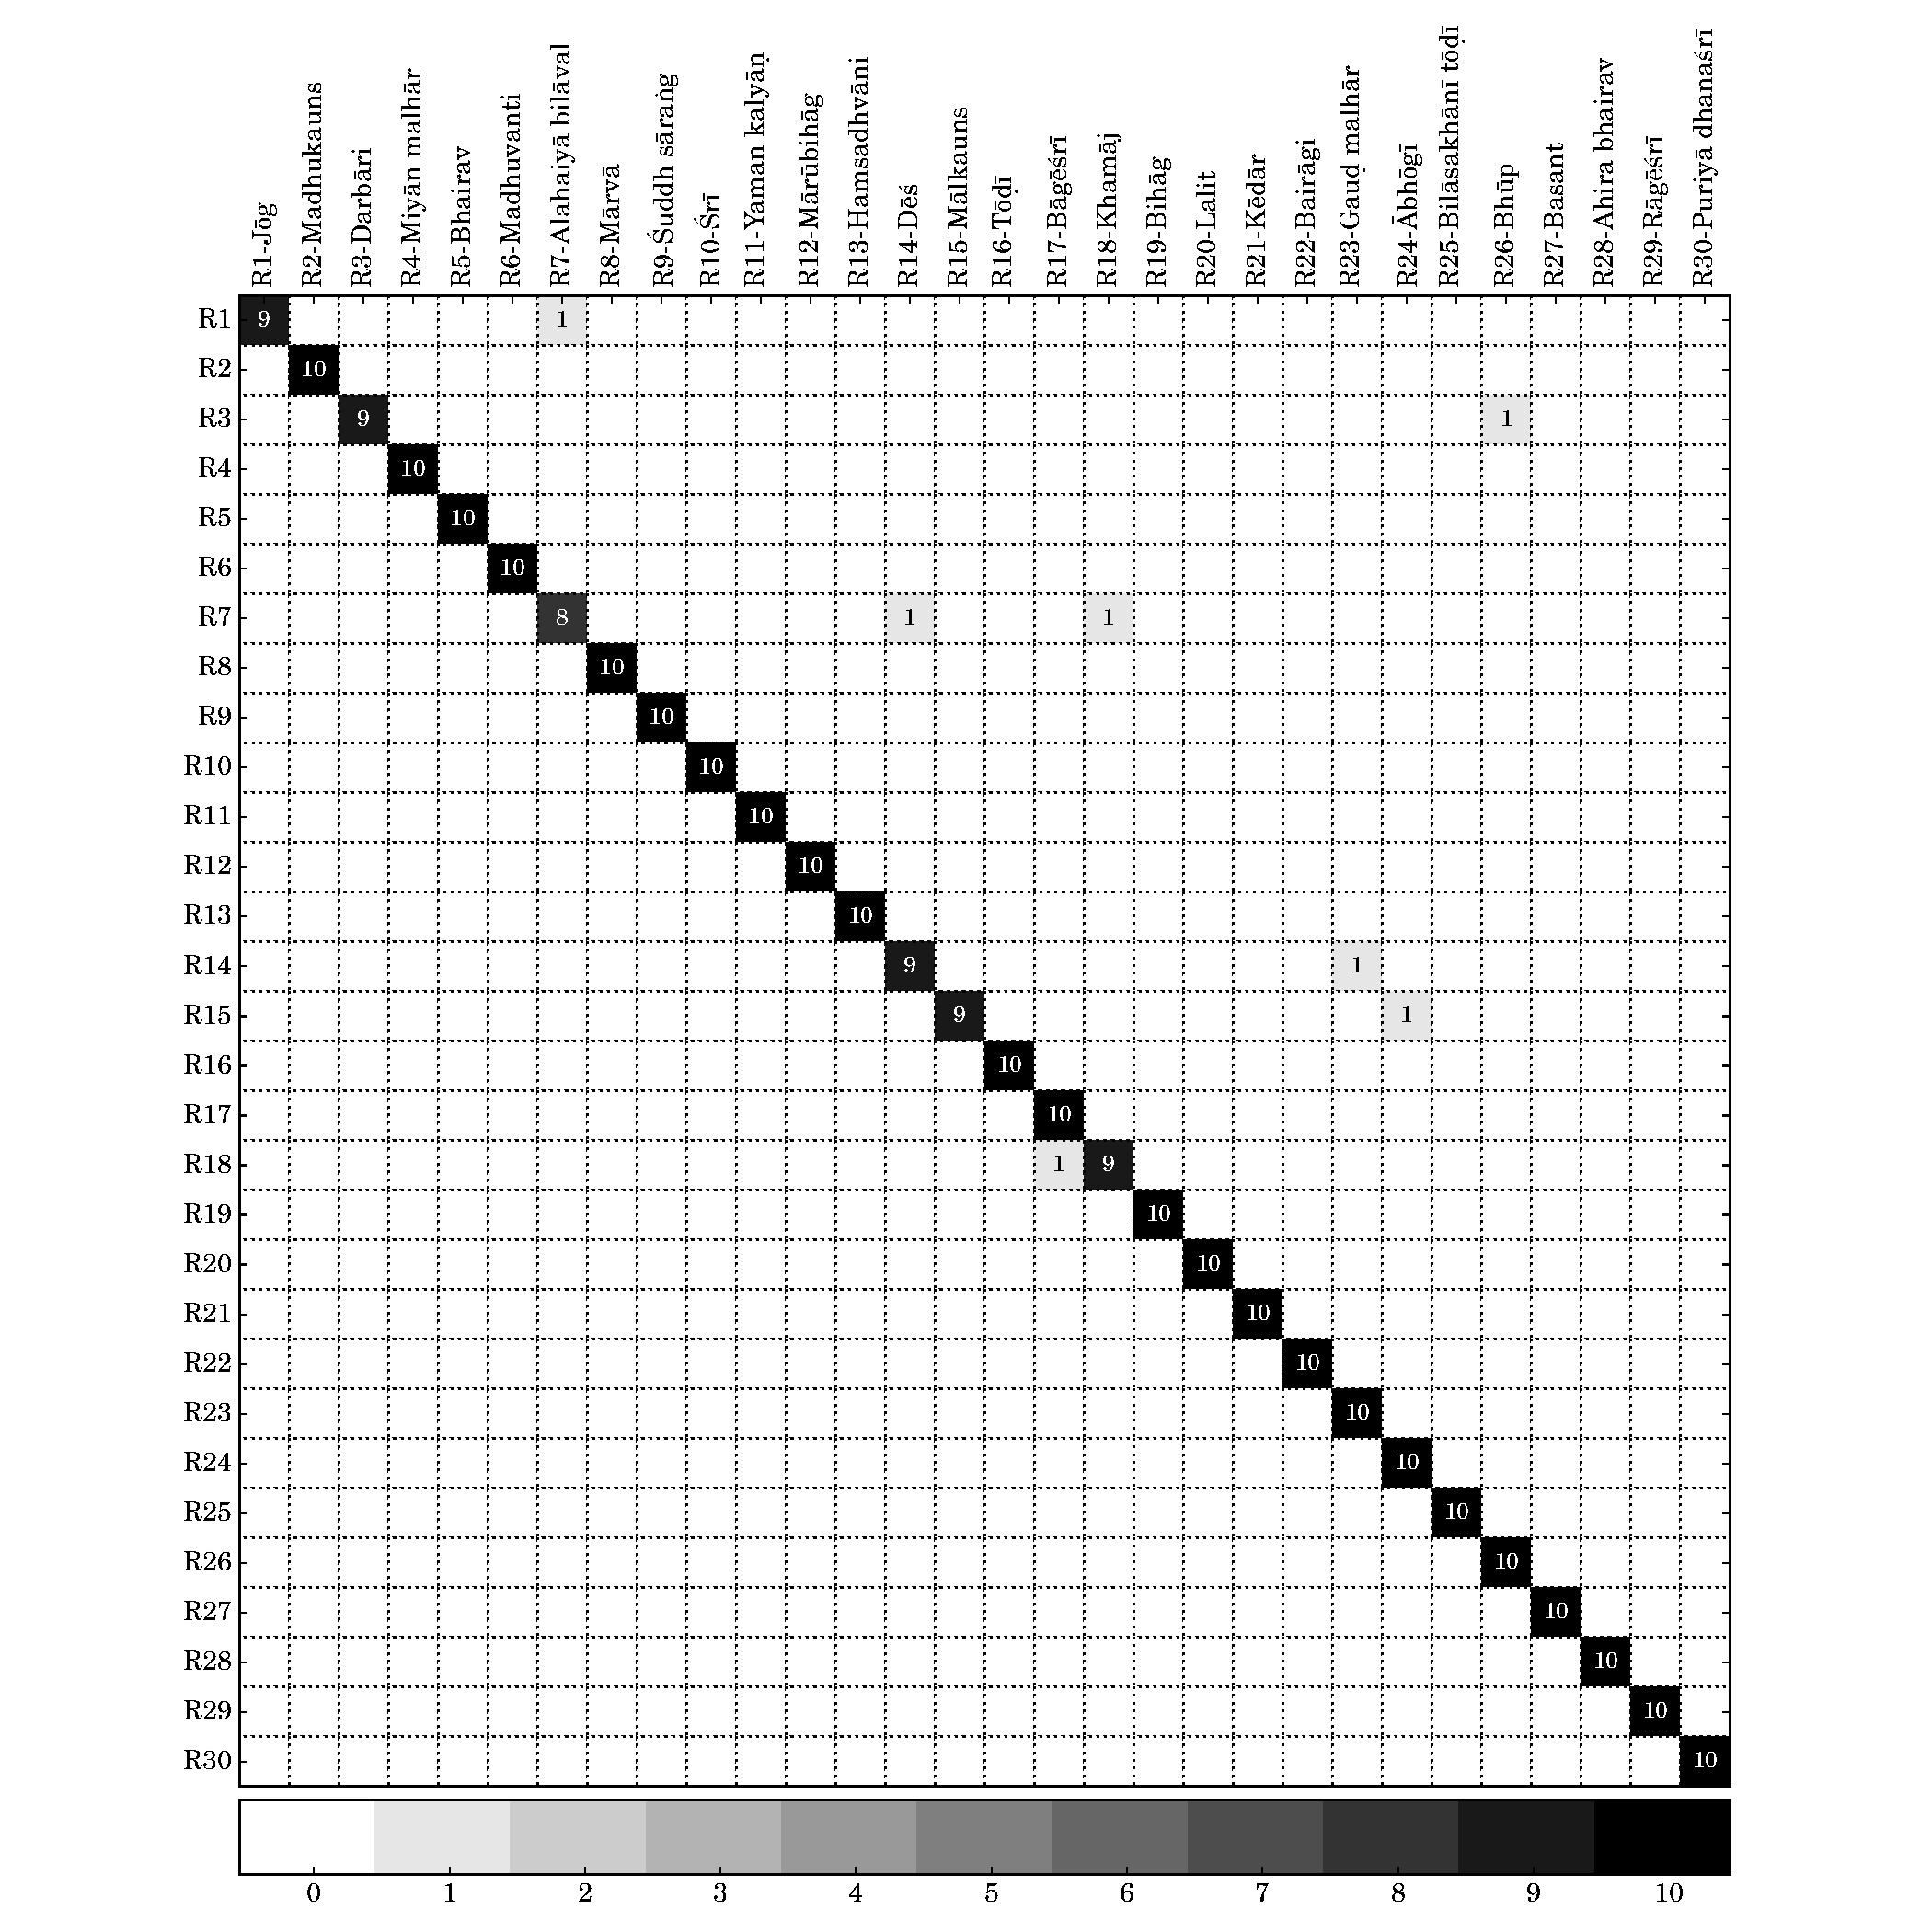
\includegraphics[width=\figSizeHundred]{ch07_ragaRecognition/figures/CM_tdms_hmd_var1.pdf}
	\end{center}
	\caption[Confusion matrix of the classification results by \acrshort{ragarecTDMS} on \acrshort{rrds_hmd_big}]{Confusion matrix of the \gls{raga} predictions by \acrshort{ragarecTDMS} on \acrshort{rrds_hmd_big} dataset. The different shades of grey are mapped to different number of audio recordings.}
	\label{fig:confusion_matrix_hmd_tdms}
\end{figure}


\begin{sidewaystable}
	\begin{threeparttable} 
		\ra{1.3}
		\begin{centering}
			\begin{tabular}{L{3cm} | L{4cm}  : L{2.5cm} | L{3cm} : L{2.5cm} | L{2.5cm}}
\tabletop				
%				\Gls{svara} full/short form & \Gls{svara} variant (Carnatic) & Notation (Carnatic) & \Gls{svara} variant (Hindustani) & Notation (Hindustani) & Position (w.r.t. Tonic)\tabularnewline
\multirow{2}{3cm}{\centering \Gls{svara} (full / short name)} & \multicolumn{2}{c |}{Carnatic music} & \multicolumn{2}{c|}{Hindustani music} & \multirow{2}{2.5cm}{\centering Position (w.r.t. the tonic)}\tabularnewline
& \Gls{svara} variant  & Notation & \Gls{svara} variant & Notation  & \tabularnewline
\tablemid				
				\Gls{shadja} (Sa) & \Gls{shadja} & S & \Gls{shadja} & S & 0\tabularnewline
\cdashline{1-6}				
				\multirow{2}{*}{\Gls{rishabha} (Re)} & \'Suddha \gls{rishabha} & R1 & K\={o}mal \gls{rishabha} & r & 1\tabularnewline
			
				& Chatu\'sruti \gls{rishabha} & R2/G1 & \'Suddha \gls{rishabha} & R & 2\tabularnewline
\cdashline{1-6}							
				\multirow{2}{*}{\Gls{gandhara} (Ga)} & S\={a}dh\={a}ra\d{n}a  \gls{gandhara} & G2/R3 & K\={o}mal \gls{gandhara} & g & 3\tabularnewline

				& Antara \gls{gandhara} & G3 & \'Suddha \gls{gandhara} & G & 4\tabularnewline
\cdashline{1-6}							
				\multirow{2}{*}{\Gls{madhyama} (Ma)} & \'Suddha \gls{madhyama} & M1 & \'Suddha \gls{madhyama} & m & 5\tabularnewline

				& Prati \gls{madhyama} & M2 & T\={\i}vra \gls{madhyama} & M & 6\tabularnewline
\cdashline{1-6}								
				\Gls{panchama} (Pa) & \Gls{panchama} & P & \Gls{panchama} & P & 7\tabularnewline
\cdashline{1-6}							
				\multirow{2}{*}{\Gls{dhaivata} (Dha)} & \'Suddha \gls{dhaivata} & D1 & K\={o}mal \gls{dhaivata} & d & 8\tabularnewline
	
				& Chatu\'sruti \gls{dhaivata} & D2/N1 & \'Suddha \gls{dhaivata} & D & 9\tabularnewline
\cdashline{1-6}							
				\multirow{2}{*}{\Gls{nishada} (\gls{ni})} & Kai\'sik\={\i} \gls{nishada} & N2/D3 & K\={o}mal \gls{nishada} & n & 10\tabularnewline

				& K\={a}kal\={\i}  \gls{nishada} & N3 & \'Suddha \gls{nishada} & N & 11\tabularnewline
\tablebot				
			\end{tabular}
			\par \end{centering}		
		\begin{tablenotes}
		\end{tablenotes}
		\caption[\Gls{svara} names and notations used in Carnatic and Hindustani music]{\Gls{svara} names and notations used in Carnatic and Hindustani music. The precise frequency and the intonation of these \glspl{svara} depend on the tonic of the lead artist in the recording and on the \gls{raga}. Note that in Carnatic music, for some \gls{svara} positions, there are two possible notations. One of these notations is used in the context of a given music piece, the selection of which depends on the \gls{raga} of the piece.}
		\label{tab:svara_notation}
	\end{threeparttable}
\end{sidewaystable}

\begin{table} 
\ra{1.2}
\centering
		\begin{tabular}{ l : L{0.4cm} : L{0.4cm} : L{0.4cm} : L{0.4cm} : L{0.4cm} : L{0.4cm} : L{0.4cm} : L{0.4cm} : L{0.4cm} : L{0.4cm} : L{0.4cm} : L{0.4cm} :}
		%\begin{tabular}{ c | c : c : c : c : c : c : c : c : c : c : c : c  }
\tabletop
			\Gls{raga} & S & r & R & g & G & m & M & P & d & D & n & N\tabularnewline
\tablemid
			\gls{jog} & $\bullet$ &  &  & $\bullet$ & $\bullet$ & $\bullet$ &  & $\bullet$&  &  & $\bullet$& \tabularnewline
		\cdashline{2-13}
			\gls{madhukauns} & $\bullet$ &  &  & $\bullet$ &  &  & $\bullet$ & $\bullet$&  &  & $\bullet$& \tabularnewline
		\cdashline{2-13}
			\gls{darbari} & $\bullet$ &  & $\bullet$ & $\bullet$ &  & $\bullet$ &  & $\bullet$& $\bullet$&  & $\bullet$& \tabularnewline
		\cdashline{2-13}
			\gls{miyan_malhar} & $\bullet$ &  & $\bullet$ & $\bullet$ &  & $\bullet$ &  & $\bullet$ &  & $\bullet$ & $\bullet$& $\bullet$\tabularnewline
		\cdashline{2-13}
			\gls{bhairav} & $\bullet$ & $\bullet$ &  &  & $\bullet$ & $\bullet$ &  & $\bullet$& $\bullet$&  &  & $\bullet$ \tabularnewline
		\cdashline{2-13}
			\gls{madhuvanti} & $\bullet$ &  & $\bullet$ & $\bullet$ &  &  & $\bullet$ & $\bullet$&  & $\bullet$&  & $\bullet$ \tabularnewline
		\cdashline{2-13}
			\gls{alahaiya_bilaval} & $\bullet$ &  & $\bullet$ &  & $\bullet$ & $\bullet$ &  & $\bullet$&  & $\bullet$& $\bullet$& $\bullet$ \tabularnewline
		\cdashline{2-13}
			\gls{marva} & $\bullet$ & $\bullet$ &  &  & $\bullet$ &  & $\bullet$ &  &  & $\bullet$&  & $\bullet$ \tabularnewline
		\cdashline{2-13}
			\gls{suddh_sarang} & $\bullet$ &  & $\bullet$ &  &  & $\bullet$ & $\bullet$ & $\bullet$&  & $\bullet$&  & $\bullet$ \tabularnewline
		\cdashline{2-13}
			\gls{sri} & $\bullet$ & $\bullet$ &  &  & $\bullet$ &  & $\bullet$& $\bullet$& $\bullet$&  &  & $\bullet$ \tabularnewline
		\cdashline{2-13}
			\gls{yaman_kalyan} & $\bullet$ &  & $\bullet$ &  & $\bullet$ & $\bullet$ & $\bullet$& $\bullet$&  & $\bullet$&  & $\bullet$ \tabularnewline
		\cdashline{2-13}
			\gls{marubihag} & $\bullet$ &  & $\bullet$ &  & $\bullet$ & $\bullet$ & $\bullet$& $\bullet$&  & $\bullet$&  & $\bullet$ \tabularnewline
		\cdashline{2-13}
			\gls{hamsadhvani} & $\bullet$ &  & $\bullet$ &  & $\bullet$ &  &  & $\bullet$&  &  &  & $\bullet$ \tabularnewline
		\cdashline{2-13}
			\gls{des} & $\bullet$ &  & $\bullet$ &  & $\bullet$ & $\bullet$ &  & $\bullet$&  & $\bullet$& $\bullet$& $\bullet$ \tabularnewline
		\cdashline{2-13}
			\gls{malkauns} & $\bullet$ &  &  & $\bullet$ &  & $\bullet$ &  &  & $\bullet$&  & $\bullet$& \tabularnewline
		\cdashline{2-13}
			\gls{todi} & $\bullet$ & $\bullet$ &  & $\bullet$ &  &  & $\bullet$& $\bullet$& $\bullet$&  &  & $\bullet$ \tabularnewline
		\cdashline{2-13}
			\gls{bagesri} & $\bullet$ &  & $\bullet$ & $\bullet$ &  & $\bullet$ &  & $\bullet$&  & $\bullet$& $\bullet$& \tabularnewline
		\cdashline{2-13}
			\gls{khamaj} & $\bullet$ &  & $\bullet$ &  & $\bullet$ & $\bullet$ &  & $\bullet$&  & $\bullet$& $\bullet$& $\bullet$ \tabularnewline
		\cdashline{2-13}
			\gls{bihag} & $\bullet$ &  & $\bullet$ &  & $\bullet$ & $\bullet$ & $\bullet$& $\bullet$&  & $\bullet$&  & $\bullet$ \tabularnewline
		\cdashline{2-13}
			\gls{lalit} & $\bullet$ & $\bullet$ &  &  & $\bullet$ & $\bullet$ & $\bullet$&  & $\bullet$&  &  & $\bullet$ \tabularnewline
		\cdashline{2-13}
			\gls{kedar} & $\bullet$ &  & $\bullet$ &  & $\bullet$ & $\bullet$ & $\bullet$& $\bullet$&  & $\bullet$& $\bullet$& $\bullet$ \tabularnewline
		\cdashline{2-13}
			\gls{bairagi} & $\bullet$ & $\bullet$ &  &  &  & $\bullet$ &  & $\bullet$&  &  & $\bullet$& \tabularnewline
		\cdashline{2-13}
			\gls{gaud_malhar} & $\bullet$ &  & $\bullet$ &  & $\bullet$ & $\bullet$ &  & $\bullet$&  & $\bullet$&  & $\bullet$ \tabularnewline
		\cdashline{2-13}
			\gls{abhogi} & $\bullet$ &  & $\bullet$ & $\bullet$ &  & $\bullet$ &  &  &  & $\bullet$&  & \tabularnewline
		\cdashline{2-13}
			\gls{bilasakhani_todi} & $\bullet$ & $\bullet$ &  & $\bullet$ &  & $\bullet$ &  & $\bullet$& $\bullet$&  & $\bullet$& \tabularnewline
		\cdashline{2-13}
			\gls{bhup} & $\bullet$ &  & $\bullet$ &  & $\bullet$ &  &  & $\bullet$&  & $\bullet$&  & \tabularnewline
		\cdashline{2-13}
			\gls{basant} & $\bullet$ & $\bullet$ &  &  & $\bullet$ & $\bullet$ & $\bullet$& $\bullet$& $\bullet$&  &  & $\bullet$ \tabularnewline
		\cdashline{2-13}
			\gls{ahira_bhairav} & $\bullet$ & $\bullet$ &  &  & $\bullet$ & $\bullet$ &  & $\bullet$&  & $\bullet$& $\bullet$& \tabularnewline
		\cdashline{2-13}
			\gls{ragesri} & $\bullet$ &  & $\bullet$ &  & $\bullet$ & $\bullet$ &  &  &  & $\bullet$& $\bullet$& \tabularnewline
		\cdashline{2-13}
			\gls{puriya_dhanasri} & $\bullet$ & $\bullet$ &  &  & $\bullet$ &  & $\bullet$& $\bullet$& $\bullet$&  &  & $\bullet$\tabularnewline
\tablebot
		\end{tabular}

\caption[List of the \glspl{raga} in \acrshort{rrds_hmd_big} along with their constituent set of \glspl{svara}]{List of the \glspl{raga} in \acrshort{rrds_hmd_big} dataset along with their constituent set of \glspl{svara}. The contents of this table are verified by Kaustuv K. Ganguli, a professional musician (vocalist of Hindustani music).}
\label{tab:raga_svaras_hmd}
\end{table}

\begin{table} 
	\ra{1.2}
	\centering
\begin{tabular}{ l c c c }
\tabletop
	\Gls{raga} & Total Duration (hrs) & \#Lead Artists & \#Releases\tabularnewline
\tablemid
	\gls{jog} & 4.68 & 8 & 8\tabularnewline
	\gls{madhukauns} & 2.86 & 7 & 8\tabularnewline
	\gls{darbari} & 5.39 & 8 & 10\tabularnewline
	\gls{miyan_malhar} & 5.82 & 9 & 10\tabularnewline
	\gls{bhairav} & 3.28 & 5 & 6\tabularnewline
	\gls{madhuvanti} & 4.01 & 10 & 8\tabularnewline
	\gls{alahaiya_bilaval} & 3.02 & 7 & 8\tabularnewline
	\gls{marva} & 4.06 & 9 & 10\tabularnewline
	\gls{suddh_sarang} & 2.66 & 8 & 8\tabularnewline
	\gls{sri} & 6.1 & 7 & 8\tabularnewline
	\gls{yaman_kalyan} & 4.2 & 9 & 10\tabularnewline
	\gls{marubihag} & 4.15 & 7 & 8\tabularnewline
	\gls{hamsadhvani} & 2.41 & 6 & 6\tabularnewline
	\gls{des} & 2.19 & 5 & 7\tabularnewline
	\gls{malkauns} & 5.89 & 13 & 10\tabularnewline
	\gls{todi} & 4.97 & 13 & 10\tabularnewline
	\gls{bagesri} & 4.86 & 10 & 10\tabularnewline
	\gls{khamaj} & 2.52 & 2 & 4\tabularnewline
	\gls{bihag} & 4.04 & 5 & 5\tabularnewline
	\gls{lalit} & 5.29 & 9 & 8\tabularnewline
	\gls{kedar} & 3.32 & 6 & 6\tabularnewline
	\gls{bairagi} & 3.09 & 7 & 8\tabularnewline
	\gls{gaud_malhar} & 4.33 & 8 & 8\tabularnewline
	\gls{abhogi} & 3.3 & 9 & 9\tabularnewline
	\gls{bilasakhani_todi} & 3.79 & 9 & 10\tabularnewline
	\gls{bhup} & 3.49 & 7 & 8\tabularnewline
	\gls{basant} & 2.74 & 9 & 10\tabularnewline
	\gls{ahira_bhairav} & 3.14 & 9 & 10\tabularnewline
	\gls{ragesri} & 3.35 & 5 & 6\tabularnewline
	\gls{puriya_dhanasri} & 3.23 & 11 & 10\tabularnewline
\tablemid
	Total & 116.2 & 60 & 162\tabularnewline
\tablebot
\end{tabular}
\caption[Details of \acrshort{rrds_hmd_big} dataset for each constituent \gls{raga}]{Details of \acrshort{rrds_hmd_big} dataset for each constituent \gls{raga} in terms of the total duration, the number of unique lead artists and the total releases associated with the audio recordings in the collection. There are 10 recordings for every \gls{raga} in this dataset.}
\label{tab:per_raga_stats_hmd}
\end{table}


\begin{table} 
	\centering
	\small
	\ra{1.1}
	\begin{tabular}{ l : L{0.17cm} : L{0.31cm} : L{0.31cm} : L{0.82cm} : L{0.31cm} : L{0.31cm} : L{0.31cm} : L{0.17cm} : L{0.31cm} : L{0.82cm} : L{0.82cm} : L{0.31cm}: }
		%\begin{tabular}{ c | c : c : c : c : c : c : c : c : c : c : c : c  }
\tabletop
			\Gls{raga} & S & R1 & R2 & G2/R3 & G3 & M1 & M2 & P & D1 & D2/N1 & N2/D3 & N3\tabularnewline
\tablemid
			\gls{sanmukhapriya} & $\bullet$ &  & $\bullet$ & $\bullet$ &  &  & $\bullet$ & $\bullet$ & $\bullet$ &  & $\bullet$ & \tabularnewline
			\cdashline{2-13}
			\gls{kapi} & $\bullet$ &  & $\bullet$ & $\bullet$ & $\bullet$  & $\bullet$ &  & $\bullet$ &  & $\bullet$ & $\bullet$ & $\bullet$\tabularnewline
			\cdashline{2-13}
			\gls{bhairavi} & $\bullet$ &  & $\bullet$ & $\bullet$ &  & $\bullet$ & & $\bullet$ & $\bullet$ & $\bullet$ & $\bullet$ & \tabularnewline
			\cdashline{2-13}
			\gls{madhyamavati} & $\bullet$ &  & $\bullet$ &  &  & $\bullet$ &  & $\bullet$ &  &  & $\bullet$ & \tabularnewline
			\cdashline{2-13}
			\gls{bilahari} & $\bullet$ &  & $\bullet$ &  & $\bullet$ & $\bullet$ &  & $\bullet$ &  & $\bullet$ &  & $\bullet$\tabularnewline
			\cdashline{2-13}
			\gls{mohanam} & $\bullet$ &  & $\bullet$ &  & $\bullet$ &  &  & $\bullet$ &  & $\bullet$ &  & \tabularnewline
			\cdashline{2-13}
			\gls{sencurutti} & $\bullet$ &  & $\bullet$ &  & $\bullet$ & $\bullet$ &  & $\bullet$ &  & $\bullet$ & $\bullet$ & \tabularnewline
			\cdashline{2-13}
			\gls{sriranjani} & $\bullet$ &  & $\bullet$ & $\bullet$ &  & $\bullet$ &  &  &  & $\bullet$ & $\bullet$ & \tabularnewline
			\cdashline{2-13}
			\gls{ritigaula} & $\bullet$ &  & $\bullet$ & $\bullet$ &  & $\bullet$ &  & $\bullet$ &  & $\bullet$ & $\bullet$ & \tabularnewline
			\cdashline{2-13}
			\gls{husseni} & $\bullet$ &  & $\bullet$ & $\bullet$ &  & $\bullet$ &  & $\bullet$ & $\bullet$ & $\bullet$ & $\bullet$ & \tabularnewline
			\cdashline{2-13}
			\gls{dhanyasi} & $\bullet$ & $\bullet$ &  & $\bullet$ &  & $\bullet$ &  & $\bullet$ & $\bullet$ &  & $\bullet$ & \tabularnewline
			\cdashline{2-13}
			\gls{atana} & $\bullet$ &  & $\bullet$ &  & $\bullet$ & $\bullet$ &  & $\bullet$ &  & $\bullet$ & $\bullet$ & $\bullet$ \tabularnewline
			\cdashline{2-13}
			\gls{behag} & $\bullet$ &  & $\bullet$ &  & $\bullet$ & $\bullet$ & $\bullet$ & $\bullet$ &  & $\bullet$ &  & $\bullet$\tabularnewline
			\cdashline{2-13}
			\gls{surati} & $\bullet$ &  & $\bullet$ &  & $\bullet$ & $\bullet$ &  & $\bullet$ &  & $\bullet$ & $\bullet$ & \tabularnewline
			\cdashline{2-13}
			\gls{kamavardani} & $\bullet$ & $\bullet$ &  &  & $\bullet$ &  & $\bullet$ & $\bullet$ & $\bullet$ &  &  & $\bullet$\tabularnewline
			\cdashline{2-13}
			\gls{mukhari} & $\bullet$ &  & $\bullet$ & $\bullet$ &  & $\bullet$ &  & $\bullet$ & $\bullet$ & $\bullet$ & $\bullet$ & \tabularnewline
			\cdashline{2-13}
			\gls{sindhubhairavi} & $\bullet$ & $\bullet$ & $\bullet$ & $\bullet$ & $\bullet$  & $\bullet$ & $\bullet$ & $\bullet$ & $\bullet$ &$\bullet$ & $\bullet$ &  $\bullet$ \tabularnewline
			\cdashline{2-13}
			\gls{sahana} & $\bullet$ &  & $\bullet$ &  & $\bullet$ & $\bullet$ &  & $\bullet$ &  & $\bullet$ & $\bullet$ & \tabularnewline
			\cdashline{2-13}
			\gls{kanada} & $\bullet$ &  & $\bullet$ & $\bullet$ &  & $\bullet$ &  & $\bullet$ &  & $\bullet$ & $\bullet$ & \tabularnewline
			\cdashline{2-13}
			\gls{mayamalavagaula} & $\bullet$ & $\bullet$ &  &  & $\bullet$ & $\bullet$ &  & $\bullet$ & $\bullet$ &  &  & $\bullet$\tabularnewline
			\cdashline{2-13}
			\gls{nata} & $\bullet$ &  &  & $\bullet$ & $\bullet$ & $\bullet$ &  & $\bullet$ &  &  &  & $\bullet$\tabularnewline
			\cdashline{2-13}
			\gls{sankarabharanam} & $\bullet$ &  & $\bullet$ &  & $\bullet$ & $\bullet$ &  & $\bullet$ &  & $\bullet$ &  & $\bullet$\tabularnewline
			\cdashline{2-13}
			\gls{saveri} & $\bullet$ & $\bullet$ &  &  & $\bullet$ & $\bullet$ &  & $\bullet$ & $\bullet$ &  &  & $\bullet$ \tabularnewline
			\cdashline{2-13}
			\gls{kamas} & $\bullet$ &  & $\bullet$ &  & $\bullet$ & $\bullet$ &  & $\bullet$ &  & $\bullet$ & $\bullet$ & \tabularnewline
			\cdashline{2-13}
			\gls{todi} & $\bullet$ & $\bullet$ &  & $\bullet$ &  & $\bullet$ &  & $\bullet$ & $\bullet$ &  &  $\bullet$  &\tabularnewline
			\cdashline{2-13}
			\gls{begada} & $\bullet$ &  & $\bullet$ &  & $\bullet$ & $\bullet$ &  & $\bullet$ &  & $\bullet$ & $\bullet$ & $\bullet$\tabularnewline
			\cdashline{2-13}
			\gls{harikambhoji} & $\bullet$ &  & $\bullet$ &  & $\bullet$ & $\bullet$ &  & $\bullet$ &  & $\bullet$ & $\bullet$ & \tabularnewline
			\cdashline{2-13}
			\gls{sri} & $\bullet$ &  & $\bullet$ & $\bullet$ &  & $\bullet$ &  & $\bullet$ &  &  $\bullet$ & $\bullet$ & \tabularnewline
			\cdashline{2-13}
			\gls{kalyani} & $\bullet$ &  & $\bullet$ &  & $\bullet$ &  & $\bullet$ & $\bullet$ &  & $\bullet$ &  & $\bullet$\tabularnewline
			\cdashline{2-13}
			\gls{saama} & $\bullet$ &  & $\bullet$ &  & $\bullet$ & $\bullet$ &  & $\bullet$ &  & $\bullet$ &  & \tabularnewline
			\cdashline{2-13}
			\gls{natakurinji} & $\bullet$ &  & $\bullet$ &  & $\bullet$ & $\bullet$ &  & $\bullet$ &  & $\bullet$ & $\bullet$ & \tabularnewline
			\cdashline{2-13}
			\gls{purvikalyani} & $\bullet$ & $\bullet$ &  &  & $\bullet$ &  & $\bullet$ & $\bullet$ &  & $\bullet$ &  & $\bullet$\tabularnewline
			\cdashline{2-13}
			\gls{yadukula_kamboji} & $\bullet$ &  & $\bullet$ &  & $\bullet$ & $\bullet$ &  & $\bullet$ &  & $\bullet$ &  $\bullet$ & \tabularnewline
			\cdashline{2-13}
			\gls{devagandhari} & $\bullet$ &  & $\bullet$ &  & $\bullet$ & $\bullet$ &  & $\bullet$ &  & $\bullet$ & $\bullet$ & $\bullet$ \tabularnewline
			\cdashline{2-13}
			\gls{kedaragaula} & $\bullet$ &  & $\bullet$ &  & $\bullet$ & $\bullet$ &  & $\bullet$ &  & $\bullet$ & $\bullet$ & \tabularnewline
			\cdashline{2-13}
			\gls{anandabhairavi} & $\bullet$ &  & $\bullet$ & $\bullet$ &  & $\bullet$ &  & $\bullet$ & $\bullet$ & $\bullet$ & $\bullet$ & \tabularnewline
			\cdashline{2-13}
			\gls{gaula} & $\bullet$ & $\bullet$ &  &  & $\bullet$ & $\bullet$ &  & $\bullet$ &  &  &  & $\bullet$\tabularnewline
			\cdashline{2-13}
			\gls{varali} & $\bullet$ & $\bullet$ &   & $\bullet$ &  &  & $\bullet$ & $\bullet$ & $\bullet$ &  &  & $\bullet$\tabularnewline
			\cdashline{2-13}
			\gls{kambhoji} & $\bullet$ &  & $\bullet$ &  & $\bullet$ & $\bullet$ &  & $\bullet$ &  & $\bullet$ & $\bullet$ & $\bullet$ \tabularnewline
			\cdashline{2-13}
			\gls{karaharapriya} & $\bullet$ &  & $\bullet$ & $\bullet$ &  & $\bullet$ &  & $\bullet$ &  & $\bullet$ & $\bullet$ & \tabularnewline
\tablebot
			\end{tabular}

	\caption[List of the \glspl{raga} in \acrshort{rrds_cmd_big} along with their constituent set of \glspl{svara}]{List of the \glspl{raga} in \acrshort{rrds_cmd_big} dataset along with their constituent set of \glspl{svara}. The \glspl{svara} are marked based on the performance practices in Carnatic music. The contents of this table are verified by Vignesh Ishwar, a professional musician (vocalist of Carnatic music).}
	\label{tab:raga_svaras_cmd}
\end{table}

\begin{table} 
	\centering
	\small
	\ra{1.1}
\begin{tabular}{l c c c}
\tabletop	
	\Gls{raga} & Total Duration (hrs) & \#Lead Artists & \#Releases\tabularnewline
\tablemid
	\gls{sanmukhapriya} & 3.05 & 12 & 12\tabularnewline
	\gls{kapi} & 1.19 & 9 & 12\tabularnewline
	\gls{bhairavi} & 5.51 & 9 & 12\tabularnewline
	\gls{madhyamavati} & 3.45 & 12 & 12\tabularnewline
	\gls{bilahari} & 3.37 & 11 & 12\tabularnewline
	\gls{mohanam} & 4.71 & 8 & 12\tabularnewline
	\gls{sencurutti} & 0.92 & 10 & 12\tabularnewline
	\gls{sriranjani} & 1.93 & 12 & 12\tabularnewline
	\gls{ritigaula} & 3.23 & 11 & 12\tabularnewline
	\gls{husseni} & 1.25 & 10 & 12\tabularnewline
	\gls{dhanyasi} & 3.37 & 8 & 12\tabularnewline
	\gls{atana} & 1.67 & 11 & 12\tabularnewline
	\gls{behag} & 1.26 & 10 & 12\tabularnewline
	\gls{surati} & 2.3 & 11 & 12\tabularnewline
	\gls{kamavardani} & 3.51 & 11 & 12\tabularnewline
	\gls{mukhari} & 3.3 & 12 & 12\tabularnewline
	\gls{sindhubhairavi} & 1.01 & 10 & 12\tabularnewline
	\gls{sahana} & 2.63 & 11 & 12\tabularnewline
	\gls{kanada} & 2.82 & 9 & 12\tabularnewline
	\gls{mayamalavagaula} & 2.58 & 11 & 12\tabularnewline
	\gls{nata} & 1.74 & 11 & 12\tabularnewline
	\gls{sankarabharanam} & 4.76 & 8 & 12\tabularnewline
	\gls{saveri} & 2.97 & 10 & 12\tabularnewline
	\gls{kamas} & 2.39 & 8 & 12\tabularnewline
	\gls{todi} & 7.23 & 9 & 12\tabularnewline
	\gls{begada} & 2.98 & 9 & 12\tabularnewline
	\gls{harikambhoji} & 3.8 & 9 & 12\tabularnewline
	\gls{sri} & 1.51 & 10 & 12\tabularnewline
	\gls{kalyani} & 5.42 & 9 & 12\tabularnewline
	\gls{saama} & 1.16 & 10 & 12\tabularnewline
	\gls{natakurinji} & 1.8 & 10 & 12\tabularnewline
	\gls{purvikalyani} & 5.87 & 9 & 12\tabularnewline
	\gls{yadukula_kamboji} & 2.13 & 11 & 12\tabularnewline
	\gls{devagandhari} & 2.27 & 11 & 12\tabularnewline
	\gls{kedaragaula} & 4.08 & 11 & 11\tabularnewline
	\gls{anandabhairavi} & 1.84 & 9 & 12\tabularnewline
	\gls{gaula} & 2.05 & 6 & 11\tabularnewline
	\gls{varali} & 3.92 & 10 & 12\tabularnewline
	\gls{kambhoji} & 6.2 & 9 & 12\tabularnewline
	\gls{karaharapriya} & 7.28 & 11 & 12\tabularnewline
\tablemid
	Total & 124.5 & 65 & 188\tabularnewline
\tablebot	
\end{tabular}
\caption[Details of \acrshort{rrds_cmd_big} dataset for each constituent \gls{raga}]{Details of \acrshort{rrds_cmd_big} dataset for each constituent \gls{raga} in terms of the total duration, the number of unique lead artists and the total releases associated with the audio recordings in the collection. There are 12 recordings for every \gls{raga} in this dataset.}
\label{tab:per_raga_stats_cmd}
\end{table}